\documentclass[notitlepage]{math}
\usepackage{lipsum}
\usetikzlibrary{patterns,positioning, decorations, decorations.pathreplacing}
\usepackage{newunicodechar}
\usepackage{amsmath}
\usepackage{centernot}


\title{Numerical Series Chap. 1} %Titre du fichie
\author{FireGhost} %Auteur du fichier


\newcommand\Warning{%
 \makebox[1.4em][c]{%
 \makebox[0pt][c]{\raisebox{.1em}{\small!}}%
 \makebox[0pt][c]{\color{red}\LARGE$\bigtriangleup$}}}%

\newunicodechar{⚠}{\Warning}

\begin{document}
\titre{Chapter 1: Numerical Series} %Titre du fichier .pdf
\UE{Numerical Series} %Nom de la UE

\fairetitre
\fairemarges
% subsubsubsection
\setcounter{secnumdepth}{4}
\titleformat{\paragraph}
{\normalfont\normalsize\bfseries}{\theparagraph}{1em}{}
\titlespacing*{\paragraph}
{0pt}{3.25ex plus 1ex minus .2ex}{1.5ex plus .2ex}



\newcommand{\minus}{\scalebox{0.75}[1.0]{$-$}} % Minus sign

\section{Preamble}
\subsection{Vocabulary}
In this chapter, we will use CVG for Convergence and DVG for Divergence. We will also use GT for General Term.
\subsection{Remark}
⚠ Be careful, the series $\sum U_n$ is not the same as the sequence $(U_n)_{n \in \mathbb{N}}$.
$\sum U_n$ is the series of general term $U_n$ and $(U_n)_{n \in \mathbb{N}}$ is the sequence $U_n$.


\section{General approach Convergence and Divergence}
\subsection{Definition}
Let $\bf(U_n)_{n \in \mathbb{N}}$ a sequence of real numbers, we call series of general term $\bf U_k$ and denote $\bf \sum U_k$ 
the sequence of partial sums $ \bf (S_n)_{n \in \mathbb{N}}$ where for any integer $\bf n \in \mathbb{N}$, $ \bf S_n = {\sum\limits_{k=0}^n U_k}$.
We say $\bf \sum U_k$ is convergent if and only if $\bf (S_n)_{n \in \mathbb{N}}$ is convergent.
\subsubsection{Example: the geometric series}
Let $\bf q \in \mathbb{R}^\star$ and let us consider the series $\bf \sum q^k$. We have:\\
\\
    $\forall n \in \mathbb{N}, S_n = \sum\limits_{k=0}^n q^k = \begin{array}{|ll}
        \frac{1 - q^{n+1}}{1 - q} & \text{if } q \neq 1  \implies
        \begin{array}{|l}
            \text{if } \minus 1 < q < 1, \sum\limits_{k=0}^{+\infty} q^k = \frac{1}{1-q} \sum U_k \text{: CVG} \\
            \text{if } q > 1 \text{ or } q < \minus 1, \sum U_k \text{: DVG} 
        \end{array} \\
        (n + 1) & \text{if } q = 1 \implies \sum U_k \text{: DVG}
    \end{array}$

\subsection{Propositions}
Let $\bf \sum U_k$ and $\bf \sum V_k$ two series of general terms and $\bf \lambda \in \mathbb{R}$. We have:
\begin{itemize}
    \item If [$\bf \sum U_k$ CVG and $\bf \sum V_k$ CVG], then $\bf \sum (U_k + V_k)$ CVG
    \item If [$\bf \sum U_k$ CVG], then $\bf \sum \lambda U_k$ CVG
    \item If [$\bf \sum U_k$ CVG and $\bf \sum V_k$ DVG], then $\bf \sum (U_k + V_k)$ DVG
    \item ⚠ $\bf \sum U_k$ DVG and $\bf \sum V_k$ DVG \underline{does not imply} $\bf \sum (U_k + V_k)$ DVG
\end{itemize}

\subsection{Sum and Remainder of a convergent series}
Let $\bf \sum U_k$ a \underline{convergent series}. We call sum of the series $\bf \sum U_k$ 
the following real number: $\bf \sum\limits_{k=0}^{+\infty} U_k = \lim\limits_{n \to +\infty} S_n$ where $\bf {S_n} = \sum\limits_{k=0}^n U_k$.
And we call remainder of the series $\bf \sum U_k$ sequence $\bf (R_n)$ defined as follows:
\[ \forall n \in \mathbb{N}, R_n = \sum\limits_{k=n+1}^{+\infty}\]
\subsubsection{Example}
$\bf \sum q^k$ CVG $\Leftrightarrow \minus 1 < q < 1$ : $\bf S = \lim\limits_{n \to +\infty} S_n = \frac{1}{1 - q}$

\subsection{Convergence necessary condition}
\subsubsection{Proposition}
Let $\bf \sum (U_k)_{k \in \mathbb{N}}$ a sequence. We have:
\[ \sum U_k \text{ CVG } \begin{array}{ r }\implies \\ \centernot{\Longleftarrow} \end{array} \left( U_k \xrightarrow[k \to +\infty]{} 0 \right) \]
\subsubsection{Example}
\begin{itemize}
    \item Harmonic series: $\bf \sum \frac{1}{n}$, $\bf (\frac{1}{n}) \xrightarrow[n \to +\infty]{} 0$ but $\bf \sum \frac{1}{n}$ DVG
    \item $\bf \sum \frac{e^n}{n^{2023}}$, $\frac{e^n}{n^{2023}} \xrightarrow[n \to +\infty]{} +\infty \implies \sum \frac{e^n}{n^{2023}}$ DVG
    \end{itemize}

\section{Positive Term Series (P.T.S.)}
\subsection{Definition}
Let $\bf \sum U_k$ a series. We say $\bf \sum U_k$ is a P.T.S., 
if and only if $\bf \forall k \in \mathbb{N}, U_k \geq 0$.\\
We say $\bf \sum U_k$ is a P.T.S. from $\bf p \in \mathbb{N}$ onwards,
if and only if $\bf \forall k \in \mathbb{N}, k \geq p \implies U_k \geq 0$.
\subsection{Propositions}
\begin{itemize}
    \item Let $\bf \sum U_k$ a P.T.S. and $\bf (S_n)_{n \in \mathbb{N}}$ the associated partial sum sequence. Then:
    \[ \sum U_k \text{ CVG } \Leftrightarrow (S_n)_{n \in \mathbb{N}} \text{ is upper-bounded} \]
    \item Let $\bf \sum U_k$ and $\bf \sum V_k$ two series such that: \\
    $\bf \forall k \in \mathbb{N}, 0 \leq U_k \leq V_k$. Then:
    \begin{enumerate}
        \item If $\bf \sum V_k$ CVG, then $\bf \sum U_k$ CVG
        \item If $\bf \sum U_k$ DVG, then $\bf \sum V_k$ DVG
    \end{enumerate}
\end{itemize}
\subsubsection{Example}
What's the nature of $\bf \sum \frac{1}{\lvert n \cdot \sin(n) \rvert}$ ?\\

\noindent $\forall n \in \mathbb{N}^\star, 0 < \lvert \sin(n) \rvert \leq 1 \implies 0 < \frac{1}{n} \leq \frac{1}{\lvert n \cdot \sin(n) \rvert}$\\
$\bf \sum \frac{1}{n}$ (Harmonic) DVG $\implies \bf \sum \frac{1}{\lvert n \cdot \sin(n) \rvert}$ DVG

\subsection{Riemann's series}
\subsubsection{Definition}
We call Riemann's series any series of General Terms (GT) $\bf \sum \frac{1}{n^\alpha}$ where $\bf \alpha \in \mathbb{R}$.\\
\subsubsection{Theorem (Riemann)}
Let $\bf \alpha \in \mathbb{R}$. Then:
\[ \sum \frac{1}{n^\alpha} \text{ CVG } \Longleftrightarrow \alpha > 1 \]
\paragraph{Example}
\begin{itemize}
    \item $\bf \sum \frac{1}{\sqrt{2}} = \sum \frac{1}{2^{\frac{1}{2}}} \implies$ DVG 
    \item $\bf \sum \frac{1 + cos(n)}{n^4}$: $\forall n \in \mathbb{N}^\star, 0 \leq 1 + cos(n) \leq 2 \implies 0 \leq \frac{1 + cos(n)}{n^4} \leq \frac{2}{n^4}$\\
    And $\bf \sum \frac{2}{n^4}$ of same nature as $\bf \sum \frac{1}{n^4}$ (Riemann's series) CVG $\implies \bf \sum \frac{1 + cos(n)}{n^4}$ CVG
\end{itemize}
\subsection{Comparison criteria}
\subsubsection{Proposition}
Let $\bf \sum U_n$ and $\bf \sum V_n$ two P.T.S.
\begin{enumerate}[label=\protect\circled{\arabic*}]
    \item If $\bf U_n \underset{+\infty}{\sim} V_n$ then $\bf \sum U_n$ and $\bf \sum V_n$ are of same nature\\
    \item If $\bf U_n = o(V_n)$ then [If $\bf \sum V_n$ CVG then $\bf \sum U_n$ CVG]
\end{enumerate}
\paragraph{Example}
What's the nature of $\bf \sum U_n$ ?
\begin{itemize}
    \item $\bf U_n = e^{-\sqrt{n}}$:
    $\begin{array}{ll}
        \text{Step 1: }& n^2 \times U_n = \frac{n^2}{e^{\sqrt{n}}} = \frac{(\sqrt{n})^4}{e^{\sqrt{n}}} \xrightarrow[n \to +\infty]{} 0 \implies U_n = o(\frac{1}{n^2})\\
        \text{Step 2: }& \sum \frac{1}{n^2} \text{ CVG (Riemann's series } \alpha = 2 > 1 \text{ )} \implies \sum U_n \text{ CVG}
    \end{array}$\\ [\bigskipamount]
    \item $\bf U_n = \ln(\frac{n+1}{n})$:
    $\begin{array}[]{l}
         \forall n \in \mathbb{N}^\star, \frac{n+1}{n} = 1 + \frac{1}{n}
         \implies  \ln(1 + \frac{1}{n}) \underset{+\infty}{=} \frac{1}{n} + o(\frac{1}{n})\\[\bigskipamount]
        ⚠ \implies 
        \begin{array}{|ll}
            \circled{1} & \forall n \in \mathbb{N}, U_n > 0 \text{ since } 1 + \frac{1}{n} > 1\\
            \circled{2} & U_n \underset{+\infty}{=} \frac{1}{n}
        \end{array}\\[\bigskipamount]
        \implies \sum U_n \text{ and } \sum \frac{1}{n} \text{ of same nature} \\
        \text{and } \sum \frac{1}{n} \text{ DVG (Harmonic series)}\\
    \end{array}$
\end{itemize}
\subsubsection{Proposition}
Let $\bf \sum U_n$ a numerical sequence. We have:\\
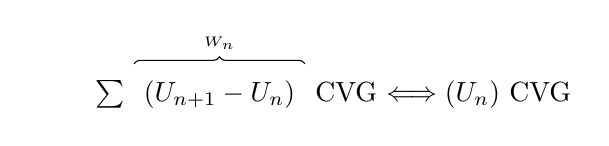
\begin{tikzpicture}[node distance=1mm]
    \node (Let) at (-2, 0) {};

    \node[above right = -0.3cm and 0.5cm of Let] (domain) {$\sum$};
    \node[right = -0.1mm of domain] (codomain) {$(U_{n+1} - U_n)$};
    \node[right = 0.1mm of codomain] (Rcodomain) {CVG $\Longleftrightarrow (U_n)$ CVG};
    \draw [decorate, decoration={brace, raise=2.5pt}] (codomain.north west) -- (codomain.north east) node [ midway,sloped,above = 0.15cm] {\tiny $W_n$};
    
\end{tikzpicture}

\paragraph{Example}
\begin{enumerate}
    \item ⚠ General Example, limit calculation:
     \begin{align*}
        \bf S_n = \sum\limits_{k=0}^{n} W_k = \sum\limits_{k=0}^n \left(U_{k+1} - U_k\right) &= \sum\limits_{k=0}^n U_{k+1} - \sum\limits_{k=0}^n U_k\\
        &= \sum\limits_{k=1}^{n+1} U_k - \sum\limits_{k=0}^n U_k\\
        &= \left(\sum\limits_{k=1}^{n} U_k + U_{n+1}\right) - \left(U_0 + \sum\limits_{k=1}^n U_k\right)\\
        Sn & = \sum\limits_{k=0}^n \left(U_{k+1} - U_k \right) = U_{n+1} - U_0
        \end{align*}
    \item 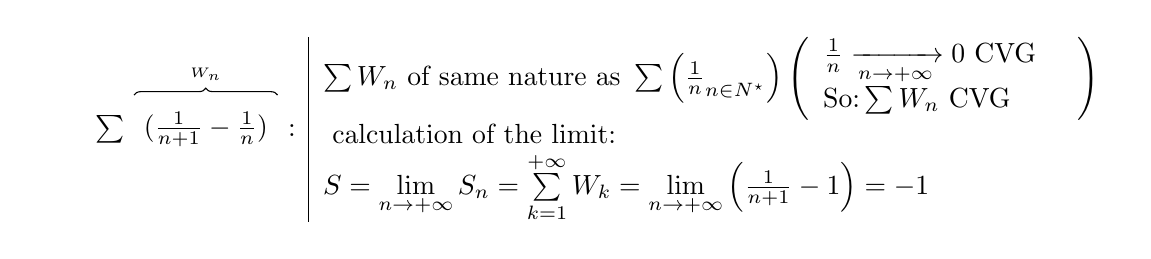
\begin{tikzpicture}[node distance=1mm]
        \node (Let) at (2, 0) {};
    
        \node[right = 0.5cm of Let] (domain) {$\sum$};
        \node[right = -0.1mm of domain] (codomain) {$(\frac{1}{n+1}-\frac{1}{n})$};
        \node[right = 0.1mm of codomain] (Rcodomain) {: $\begin{array}{|l}
        \sum W_n \text{ of same nature as } \sum \left(\frac{1}{n}_{n \in \mathbb{N}^\star}\right) \left( \begin{array}{ll}
            \frac{1}{n} \xrightarrow[n \to +\infty]{} 0 \text{ CVG}&\\
            \text{So:}  \sum W_n \text{ CVG}&
        \end{array} \right)\\
        \text{ calculation of the limit: }\\
        S = \lim\limits_{n \to +\infty} S_n = \sum\limits_{k=1}^{ +\infty} W_k = \lim\limits_{n \to +\infty} \left(\frac{1}{n+1} - 1\right) = -1
        \end{array}$};
    
        \draw [decorate, decoration={brace, raise=2.5pt}] (codomain.north west) -- (codomain.north east) node [ midway,sloped,above = 0.15cm] {\tiny $W_n$};
    \end{tikzpicture}
    
\end{enumerate}
\subsection{Riemann's Rule}
Let $\bf \sum U_n$ a \underline{Positive} numerical series.
If $\bf \exists \alpha > 1 , n^\alpha \times U_n \underset{+\infty}{\sim} 0$ then $\bf \sum U_n$ CVG
\subsubsection{Proof}
$\bf \exists \alpha > 1, n^\alpha \times U_n \xrightarrow[n \to +\infty]{} 0 \implies \frac{U_n}{\frac{1}{n^\alpha}} \xrightarrow[n \to +\infty]{} 0$\\
$\implies \left\{ \begin{array}{r|r}
    U_n = o(\frac{1}{n^\alpha}) &\\
    \text{and } &\\ 
    \alpha > 1 & \left[ \sum \frac{1}{n^\alpha} \text{ CVG (Riemann's series)} \implies \sum U_n \text{ CVG} \right]\\
    \text{and } &\\
    \sum U_n \text{ P.T.S.}& \\
\end{array} \right. $
\subsection{D'Alembert's Rule (Ratio Test)}
Let $\bf (U_n)$ be a strictly positive sequence such that:
\[ \frac{U_{n+1}}{U_n} \xrightarrow[n \to +\infty]{} \ell \in \mathbb{R}_+\cup \{+\infty\} \]
Then:
$\begin{array}{l}
    \ell < 1 \implies \sum U_n \text{ CVG}\\
    \ell > 1 \implies \sum U_n \text{ DVG}\\
    \ell = 1 \implies \text{ no conclusion}    
\end{array}$
\subsubsection{Example}
$\bf \sum \frac{1}{n!}$ : $\forall n \in \mathbb{N}, \frac{1}{n!} > 0$ (P.T.S.) and $\frac{U_{n+1}}{U_n} = \frac{\frac{1}{(n+1)!}}{\frac{1}{n!}} = \frac{1}{n+1} \xrightarrow[n \to +\infty]{} 0 < 1 \implies \sum \frac{1}{n!}$ CVG\\

\subsection{Cauchy's Rule}
Let $\bf (U_n)$ be a strictly positive sequence such that:
\[ \sqrt[n]{U_n} \xrightarrow[n \to +\infty]{} \ell \in \mathbb{R}_+\cup \{+\infty\} \]
Then:
$\begin{array}{l}
    \ell < 1 \implies \sum U_n \text{ CVG}\\
    \ell > 1 \implies \sum U_n \text{ DVG}\\
    \ell = 1 \implies \text{ no conclusion}
\end{array}$
\subsubsection{Example}
$\bf \sum {(\frac{n}{n+1})^n}^2$: $\forall n \in \mathbb{N}, {(\frac{n}{n+1})^n}^2 > 0$ (P.T.S.), $\sqrt[n]{U_n} = \left({(\frac{n}{n+1})^n}^2\right)^{\frac{1}{n}} = (\frac{n}{n+1})^n = e^{n \ln(1 - \frac{n}{n+1})}$\\[0.2cm]
$\ln(1 - \frac{n}{n+1}) \sim n \times (-\frac{n}{n+1}) \xrightarrow[n \to +\infty]{} -1 < 0 \implies \sqrt[n]{U_n} \xrightarrow[n \to +\infty]{} e^{-1} = \frac{1}{e} < 1 \underset{\text{Cauchy}}{\implies} \sum U_n$ CVG\\
\subsection{Examples}
\begin{enumerate}[label=\protect\circled{\arabic*}]
    \item $\sum (1 + \frac{1}{n})^n$: $1 + \frac{1}{n} \centernot{\xrightarrow[n \to +\infty]{}} 0$ (don't have the necessary condition) $\implies \sum (1 + \frac{1}{n})^n$ DVG\\
    \item $\sum \left((1 + \frac{1}{n})^n - e\right)$: 
    \begin{enumerate}
        \item   \begin{align*}
             \left((1 + \frac{1}{n})^n - e\right) = e^{n \times \ln(1 + \frac{1}{n})} - e &= e^{n \times (\frac{1}{n} - \frac{1}{2n^2} + o(\frac{1}{n^2}))} - e \\
             &= e^{1 - \frac{1}{2n} + o(\frac{1}{n})} - e \\
             &= e \times e^{-\frac{1}{2n} + o(\frac{1}{n})} - e \\ &= e \times (1 - \frac{1}{2n} + o(\frac{1}{n})) - e \\ &= -\frac{e}{2n} + o(\frac{1}{n})
            \end{align*}
            So $\left((1 + \frac{1}{n})^n - e\right) \underset{+\infty}{\sim} -\frac{e}{2n}$ (Can't use P.T.S. property)
        \item $\sum -\frac{e}{2n} < 0$ for $ n \in \mathbb{N}^\star$
        \item $\exists p \in \mathbb{N}^\star, (n \geq p) \implies (\left((1 + \frac{1}{n})^n - e\right) \leq 0)$ (Same sign as $\sum -\frac{e}{2n}$) \\[0.2cm]
        $\implies \sum \left((1 + \frac{1}{n})^n - e\right)$ has the same nature as $\sum -\frac{e}{2n}$ wich is of same nature as $\sum \frac{1}{n}$ DVG
    \end{enumerate}
    \item $\sum n^{2023} \times e^{-n} = \sum \frac{n^{2023}}{e^n}$: $n^{2023} = o(e^n)$ (growth comparison)
    $n^{2025} \times e^{-n} = \frac{\frac{n^{2023}}{e^n}}{\frac{1}{n^2}} \xrightarrow[n \to +\infty]{} 0 \implies U_n = o(\frac{1}{n^2}) \underset{\text{Riemann} (\alpha = 2>1)}{\implies} \sum U_n$ CVG\\
    \item $\sum n! \times e^{-n}$\\
\end{enumerate}
\section{Alternating Series}
\subsection{Definition}
Let $\bf (U_n) \in \mathbb{R}^\mathbb{N}$, we say $\bf (U_n)$ is an alternating sequence thus $\bf \sum U_n$ an alternating series, if there exists $\begin{array}{|l} \text{a positive} \\ \color{green}\text{a negative}\end{array}$ sequence $\bf (a_n)$ such that:
\[\bf \forall n \in \mathbb{N}, \begin{array}{|l} U_{n} = (-1)^n \times a_n \\ \color{green} U_{n} = (-1)^{n+1} \times a_n \end{array}\]
\subsubsection{Example}
$\bf \sum \frac{(-1)^n}{n}$ is an alternating series because $\bf \forall n \in \mathbb{N}, \frac{(-1)^n}{n} = (-1)^n \times \frac{1}{n}$
\subsection{Alternating Series Special Criteria (A.S.S.C.)}
\subsubsection{Theorem}
Let $\bf (U_n)$ an alternating sequence, such that:
\[\bf \left. \begin{array}{l}
    U_n \xrightarrow[n \to +\infty]{} 0\\
    (\left\lvert U_n \right\rvert )_{n \in \mathbb{N}} \text{ is decreasing}
\end{array} \right] \implies \sum U_n \text{ CVG}\]
\subsubsection{Explanation}
An alternating sequence is of the form 
\begin{align*}
    \bf U_n = (-1)^n \times a_n & \qquad \text{ or } & \bf U_n = (-1)^{n+1} \times a_n\\
\bf \left\lvert U_n \right\rvert = \left\lvert (-1)^n \times a_n \right\rvert = \left\lvert a_n \right\rvert & \qquad \text{ or } & \bf \left\lvert U_{n} \right\rvert = \left\lvert (-1)^{n+1} \times a_{n} \right\rvert = \left\lvert a_{n} \right\rvert\\
\text{So }& \bf (\left\lvert U_n \right\rvert )_{n \in \mathbb{N}} = (a_n)_{n \in \mathbb{N}}&\\
\end{align*}
\section{Absolute Convergence}
\subsection{Definition}
Let $\bf (U_n)$ a sequence, we say $\bf \sum U_n$ is absolutely convergent if $\bf \sum \left\lvert U_n \right\rvert$ is convergent.
\subsubsection{Example}
$\bf \sum \frac{(-1)^n}{n^2}$ is absolutely convergent because $\bf \sum \left\lvert \frac{(-1)^n}{n^2} \right\rvert = \sum \frac{1}{n^2}$ is convergent.
\subsection{Proposition}
Let $\bf \sum U_n$ a series, if $\bf \sum U_n$ is absolutely convergent then $\bf \sum U_n$ is convergent.
\[\bf \sum \left\lvert U_n \right\rvert \text{ CVG } \begin{array}{l}  \implies \\ {\color{red}\centernot{\color{black}\Longleftarrow}} \end{array} \bf \sum U_n \text{ CVG.}\]
\subsubsection{Counter Example}
$\bf \sum \frac{(-1)^n}{n}$ is convergent BUT $\bf \sum \left\lvert \frac{(-1)^n}{n} \right\rvert = \sum \frac{1}{n}$ is divergent.
\subsection{Examples}
\subsubsection{Example 1}
\begin{itemize}
    \item $\bf \sum \frac{(-1)^n}{n^\alpha}, \alpha \in \mathbb{R}$: 
    \begin{itemize}
        \item case $\alpha \leq 0$: $\bf \sum \frac{(-1)^n}{n^\alpha} \centernot{\xrightarrow[n \to +\infty]{}} 0$ (necessary condition) $\implies \bf \sum \frac{(-1)^n}{n^\alpha}$ DVG.
        \item case $\alpha > 0$: $
             \bf \sum \frac{1}{n^\alpha} > 0 \implies \bf \sum \frac{(-1)^n}{n^\alpha} \text{ is an alternating series}.\\[1em]
            \begin{array}{l|c}
             \bf \frac{1}{n^\alpha} \xrightarrow[n \to +\infty]{} 0\\[1em]
             \bf \left\lvert \frac{1}{n^\alpha} \right\rvert = \frac{1}{n^\alpha} \text{ is decreasing}&
        \end{array}$ $\overset{\text{A.S.S.C.}}{\implies} \bf \sum \frac{(-1)^n}{n^\alpha}$ CVG.
    \end{itemize}
\end{itemize}
\paragraph{Proposition deduced from example 1}
$\bf \forall \alpha > 0, \sum \frac{(-1)^n}{n^\alpha}$ is convergent.
\subsubsection{Example 2}
\begin{itemize}
    \item $\bf \forall n \in \mathbb{N}, U_n = \frac{\sin(n)}{n^\alpha}$:
    $\bf \left\lvert U_n \right\rvert = \frac{\left\lvert \sin(n) \right\rvert}{n^\alpha}, \implies 0 \leq \left\lvert U_n \right\rvert \leq \frac{1}{n^\alpha}$\\[1em]
    \begin{align*}
        \text{If } \bf \alpha > 1, &\text{ then } \sum \frac{1}{n^\alpha} \text{ CVG (Riemann }\alpha > 1\text{)}\\
        &\text{ then } \sum \left\lvert U_n \right\rvert \text{ CVG (Comparison test)}\\
        &\text{ then } \sum U_n \text{ Absolutely CVG (Proposition)}\\
        &\text{ then } \sum U_n \text{ CVG (Proposition)}
    \end{align*}

\end{itemize}

\newpage
\section{Important Proof}
\subsection{Series whose general term is positive}
\fbox{
\begin{minipage}{0.9\textwidth}   
    \subsubsection{Theorem (Comparison rules)}
    Consider two sequences $\bf (U_n)$ and $\bf (V_n)$.
    \begin{enumerate}
        \item If for all $n \in \mathbb{N}, u_n \leq v_n$, then
        \begin{enumerate}
            \item $\bf \sum v_n$ converges $\implies \sum u_n$ converges
            \item $\bf \sum u_n$ diverges $\implies \sum v_n$ diverges
        \end{enumerate}
        If $\bf u_n \sim v_n$ then the series $\bf \sum u_n$ and $\bf \sum v_n$ have the same nature.
    \end{enumerate}
\end{minipage}}
\paragraph{Remarks}
\begin{itemize}[label={--}]
    \item Property 1 remains true if the relation $\bf u_n \leq v_n$ satisfied only above a certain rank, instead of for all $n \in \mathbb{N}$.
    That is, it is true if there exists  $n_0 \in \mathbb{N}$ such that
    \[ \forall n \in \mathbb{N}, n \geq n_0 \implies u_n \leq v_n \]
    \item Property 1 includes the case $u_n = o(v_n)$.  Indeed, in this case, the relation $\bf u_n \leq v_n$ is satisfied above a certain rank.
\end{itemize}
\paragraph{Proof}
\begin{enumerate}
    \item Let $\bf (S_n)$ denote the partial sums of $\bf \sum u_n$ and $\bf (T_n)$ the partial sums of $\bf \sum v_n$.
    To start with, note that the sequences $\bf (S_n)$ and $\bf (T_n)$ are both increasing. Indeed, for all $n \in \mathbb{N}$,
    \[ S_{n+1} - S_n = u_{n+1} \geq 0 \quad \text{ and } \quad T_{n+1} - T_n = v_{n+1} \geq 0 \]
    Thus, we know that
    \[ (S_n) \text{ converges } \Longleftrightarrow (S_n) \text{ is bounded above} \]
    Furthermore, since for all $n \in \mathbb{N}$, $u_n \leq v_n$, we can write:
    \[ \forall n \in \mathbb{N}, \quad S_n \leq T_n \]
    Thus, if $\bf \sum v_n$ converges, then $\bf (T_n)$ is bounded.  It hence admits an upper bound $M$. Then for all $n \in \mathbb{N}$:
    \[ S_n \leq T_n \leq M \]
    and $M$ is also an upper bound of $\bf (S_n)$. The sequence $\bf (S_n)$ is hence bounded above and, since it is increasing, it converges. This proves the property (a).\\[1em]
    Proving property (b) is now straightforward: it is the contrapositive of property (a).

    \item Assume that $(u_n) \sim (v_n)$. Then there exists a sequence $(\epsilon_n)$ such that
    \[ \forall n \in \mathbb{N}, u_n = v_n \times (1 + \epsilon_n) \quad \text{ and } \quad \epsilon_n \xrightarrow[n \to +\infty]{} 0 \]
    Since $(\epsilon_n)$ converges to $0$, it remains between $-\frac{1}{2}$ and $\frac{1}{2}$ above a certain rank: there exists $n_0 \in \mathbb{N}$ such that
    \begin{align*}
        \forall n \in \mathbb{N}, n \geq n_0 &\implies -\frac{1}{2} \leq \epsilon_n \leq \frac{1}{2}\\
        &\implies \frac{1}{2} \leq 1 + \epsilon_n \leq \frac{3}{2}\\
        &\implies \frac{1}{2} v_n \leq u_n \leq \frac{3}{2} v_n
    \end{align*}
    If $\bf \sum u_n$ converges then, using property 1 and the relation $\frac{1}{2} v_n \leq u_n$, we know that $\bf \sum \frac{1}{2} v_n$ converges.
    Thus, $\bf \sum v_n$ converges.\\[1em]

    If $\bf \sum u_n$ diverges then, using property 1 and the relation $u_n \leq \frac{3}{2} v_n$, we know that $\bf \sum \frac{3}{2} v_n$ diverges.
    Thus, $\bf \sum v_n$ diverges.    
\end{enumerate}

\fbox{
\begin{minipage}{0.9\textwidth}   
    \subsubsection{Theorem (Riemann series)}
    Let $\alpha$ in $\mathbb{R}$. The series $\sum \frac{1}{n^\alpha}$ converges if and only if $\alpha > 1$.
\end{minipage}}
\paragraph{Some explanations before the proof:}
Before the explicit proof, here are the main ideas we will use:
\begin{enumerate}
    \item We focus on the case $\alpha > 0$ (otherwise, $\frac{1}{n^\alpha}$ does not converge to $0$, hence the series diverges).
    \item When $0 < \alpha \leq 1$, we try to lower-bound $\frac{1}{n^\alpha}$ by a positive sequence $\bf (v_n)$ such that $\sum v_n$ diverges.
    And when $\alpha > 1$, we try to upper-bound $\frac{1}{n^\alpha}$ by a positive sequence $\bf (w_n)$ such that $\sum w_n$ converges.
    \item In that purpose, we use the property that, since the function $t \mapsto \frac{1}{t^\alpha}$ decreases, we know that for all $n \geq 2$:
    \[ \forall t \in [n-1, n], \frac{1}{t^\alpha} \geq \frac{1}{n^\alpha} \quad \text{ and } \quad \forall t \in [n, n+1], \frac{1}{n^\alpha} \geq \frac{1}{t^\alpha} \]
    We can hence integrate the first inequality on $[n-1, n]$ and the second one on $[n, n+1]$:
    \[\int_{n-1}^n \frac{1}{t^\alpha} \mathrm{d}t \geq \int_{n-1}^n \frac{1}{n^\alpha} \mathrm{d}t \quad \text{ and } \quad \int_n^{n+1} \frac{1}{n^\alpha} \mathrm{d}t \geq \int_n^{n+1} \frac{1}{t^\alpha} \mathrm{d}t\]
    The function $t \mapsto \frac{1}{t^\alpha}$ is a constant function. Thus,
    %int 1/n^a dt = [t/n^a]_n-1^n = 1/n^a
    \[ \int_{n-1}^n \frac{1}{n^\alpha} \mathrm{d}t = \left[\frac{t}{n^\alpha}\right]_{n-1}^n = \frac{1}{n^\alpha} \quad \text{ and } \quad \int_n^{n+1} \frac{1}{n^\alpha} \mathrm{d}t = \left[\frac{t}{n^\alpha}\right]_n^{n+1} = \frac{1}{n^\alpha} \]
    Finally, for all $n \geq 2$,
    \[ \int_{n-1}^n \frac{1}{t^\alpha} \mathrm{d}t \geq \frac{1}{n^\alpha} \geq \int_n^{n+1} \frac{1}{t^\alpha} \mathrm{d}t \]
    


    \fbox{
    \begin{minipage}{0.9\textwidth}   
        \begin{center}
            
            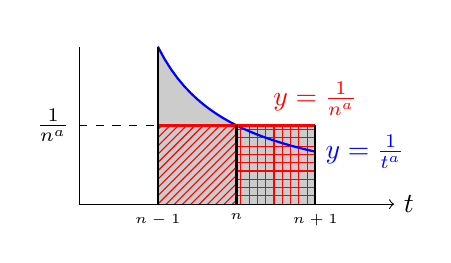
\begin{tikzpicture}[scale=2]
                %move all the tikz to the right
                %fill the surface between the curves
                \fill[gray!40, domain=0.5:1.5, variable=\x]
                (0.5,0) -- plot (\x,{(1/(\x))/2}) -- (1.5,0) -- cycle;
                \fill[gray!40, domain=0.5:1.5, variable=\x]
                (0.5,0) -- plot (\x,{0.5}) -- (1.5,0) -- cycle;
                %fill the surface bellow the red curves in the interval [0.5,1] hatch red
                \fill[pattern=north east lines, pattern color=red, domain=0.5:1, variable=\x]
                (0.5,0) -- plot (\x,{0.5}) -- (1,0) -- cycle;
                \fill[pattern=grid, pattern color=red, domain=1:1.5, variable=\x]
                (1,0) -- plot (\x,{0.5}) -- (1.5,0) -- cycle;
                
                \draw[blue, thick] plot[domain=0.5:1.5] (\x,{(1/(\x))/2}) node[right] {$y=\frac{1}{t^a}$};
                \draw[red, thick] plot[domain=0.5:1.5] (\x,{0.5}) node[right, above] {$y=\frac{1}{n^a}$};
                
                \draw[->] (0,0) -- (2,0) node[right] {$t$};
                \draw (0,0) -- (0,1) node[above] {};
                
                \draw[dashed] (0,0.5) -- (0.5,0.5);
                \draw[thick] (0.5,0) -- (0.5,1);
                \draw[thick] (1,0) -- (1,0.5);
                \draw[thick] (1.5,0) -- (1.5,0.5);
                
                \node[below] at (0.5,0) {\tiny$n-1$};
                \node[below] at (1,0) {\tiny$n$};
                \node[below] at (1.5,0) {\tiny$n+1$};
                \node[left] at (0,0.5) {$\frac{1}{n^a}$};
            \end{tikzpicture}
        \end{center}
    \end{minipage}}
    \item To compute the integral of $\frac{1}{t^\alpha}$: a primitive function $F$ is defined on $\mathbb{R}^*_+$ by:
    \[ F(t) = \frac{t^{-\alpha+1}}{-\alpha+1} \text{ (case } \alpha \neq 1 \text{)} \quad \text{ or } \quad F(t) = \ln(t) \text{ (case } \alpha = 1 \text{)} \]
\end{enumerate}
\paragraph{Theorem's proof}
Let $\alpha \in \mathbb{R}$ and the series $\sum \frac{1}{n^\alpha}$.

\begin{enumerate}
    \item If $\alpha \leq 0$, then $\frac{1}{n^\alpha} = n^{-\alpha}$ with $-\alpha \geq 0$. Thus,  $\left(\frac{1}{n^\alpha}\right)$ does not converge to $0$ and the series diverges.
    \item If $0 < \alpha \leq 1$: since the function $t \mapsto \frac{1}{t^\alpha}$ decreases on $\mathbb{R}^*_+$, we know that for all $n \geq 1$:
    \[ \forall t \in [n, n+1], \frac{1}{n^\alpha} \geq \frac{1}{t^\alpha} \]
    By integrating this inequality on $[n, n+1]$, we get: $\int_n^{n+1} \frac{1}{n^\alpha} \mathrm{d}t \geq \int_n^{n+1} \frac{1}{t^\alpha} \mathrm{d}t$.\\[0.5em]
    The first integral is $\left[\frac{t}{n^\alpha}\right]_n^{n+1} = \frac{1}{n^\alpha}$.\\[1em]
    If $F$ denotes a primitive function of $\frac{1}{t^\alpha}$, we hence get:
    \[ \forall n \geq 1, \frac{1}{n^\alpha} \geq F(n+1) - F(n) \geq 0 \]

    Since both series $\sum \frac{1}{n^\alpha}$ and $\sum \left(F(n+1) - F(n)\right)$ have positive terms, we can use comparison theorem. 
    Let us prove that the serie $\sum \left(F(n+1) - F(n)\right)$ diverges: the latter is a telescoping series, it hence has the same nature as the sequence $(F(n))$.

    If $\alpha < 1$, then for all $n \in \mathbb{N}^*$, $F(n) = \frac{n^{1-\alpha}}{1-\alpha}$ with $1-a > 0$. The sequence $(F(n))$ hence diverges to $+\infty$, that is, $\sum \left(F(n+1) - F(n)\right)$ diverges.\\[0.5em]

    If $\alpha = 1$, then for all $n \in \mathbb{N}^*$, $F(n) = \ln(n)$ and the sequence $(F(n))$ diverges to $+\infty$. Here also, $\sum \left(F(n+1) - F(n)\right)$ diverges.\\[0.5em]
    
    Finally, for all $\alpha$ such that $0 < \alpha \leq 1$, the series $\sum \left(F(n+1) - F(n)\right)$ diverges. Using comparison theorem, it results that $\sum \frac{1}{n^\alpha}$ diverges too.

    \item If $\alpha > 1$: since the function $t \mapsto \frac{1}{t^\alpha}$ decreases on $\mathbb{R}^*_+$, we know that for all $n \geq 2$:
    \[ \forall t \in [n-1, n], \frac{1}{n^\alpha} \leq \frac{1}{n^\alpha} \]

    By integrating this inequality on $[n-1, n]$, we get: $\int_{n-1}^n \frac{1}{n^\alpha} \mathrm{d}t \leq \int_{n-1}^n \frac{1}{t^\alpha} \mathrm{d}t$.\\[0.5em]
    The first integral is $\left[\frac{t}{n^\alpha}\right]_{n-1}^n = \frac{1}{n^\alpha}$.\\[1em]
    If $F$ denotes a primitive function of $\frac{1}{t^\alpha}$, we hence get:
    \[ \forall n \geq 1, 0 \leq \frac{1}{n^\alpha} \leq F(n) - F(n-1) \]

    Since both series $\sum \frac{1}{n^\alpha}$ and $\sum \left(F(n) - F(n-1)\right)$ have positive terms, we can use comparison theorem.
    Let us prove that the serie $\sum \left(F(n) - F(n-1)\right)$ converges: the latter is a telescoping series, it hence has the same nature as the sequence $(F(n))$.\\[0.5em]

    But $F(n) = \frac{n^{1-\alpha}}{1-\alpha} = -\frac{1}{(1-\alpha)} \times \frac{1}{n^{\alpha-1}}$ with $\alpha - 1 > 0$.\\

    Thus, the sequence $(F(n))$ converges to $0$ and the telescoping series $\sum \left(F(n) - F(n-1)\right)$ converges.\\[0.5em]

    Using comparison theorem, it results that $\sum \frac{1}{n^\alpha}$ converges too.
\end{enumerate}
\subsection{Series whose general term has a non-constant sign}
\fbox{
\begin{minipage}{0.9\textwidth}   
    \subsubsection{Theorem (Absolute convergence)}
    If a series $\sum u_n$ converges absolutely, then it converges.
\end{minipage}}\\[1em]
{\color{blue} Reminder: a series $\sum u_n$ converges absolutely if $\sum \left\lvert u_n \right\rvert$ converges.}
\paragraph{Proof}
\noindent Consider a series $\sum u_n$ converging absolutely. We hence assume that $\sum \left\lvert u_n \right\rvert$ converges.\\[0.5em]
Let us define the two series $(u_n^+)$ and $(u_n^-)$ by:
\[ \forall n \in \mathbb{N}, \quad u_n^+ = \begin{cases}
    u_n & \text{ if } u_n \geq 0\\
    0 & \text{ otherwise}
\end{cases} \quad \text{ and } \quad u_n^- = \begin{cases}
    -u_n & \text{ if } u_n \leq 0\\
    0 & \text{ otherwise}
\end{cases} \]

\noindent These sequences are both positive $u_n = u_n^+ - u_n^-$. Furthermore, 
\begin{itemize}
    \item[--] $\forall n \in \mathbb{N}, 0 \leq u_n^+ \leq \left\lvert u_n \right\rvert$ and $\sum \left\lvert u_n \right\rvert$ converges, so $\sum u_n^+$ converges.
    \item[--] $\forall n \in \mathbb{N}, 0 \leq u_n^- \leq \left\lvert u_n \right\rvert$ and $\sum \left\lvert u_n \right\rvert$ converges, so $\sum u_n^-$ converges.
\end{itemize}
Thus, $\sum u_n = \sum \left(u_n^+ - u_n^-\right)$ is the sum of two convergent series. It is hence convergent.\\[1em]

\fbox{
\begin{minipage}{0.9\textwidth}   
    \subsubsection{Theorem (Leibniz's rule)}
    Let $(u_n)$ be an alternating sequence. If $(\left\lvert u_n \right\rvert)$ is decreasing and converges to $0$, then:
    \begin{enumerate}
        \item $\sum u_n$ converges.
        \item The remainder $(R_n)$ of the series satisfy to: $\forall n \in \mathbb{N}, \left\lvert R_n \right\rvert \leq \left\lvert u_{n+1} \right\rvert$.
    \end{enumerate}
\end{minipage}}

\paragraph{Reminders}
the theorem's proof relies on the notion of adjacent sequences and on two properties seen during the chapter 5 (sequences) the previous year:
\begin{enumerate}
    \item Two sequences $(u_n)$ and $(v_n)$ are adjacent if they satisfy the conditions:
    \begin{itemize}
        \item[--] One of them is increasing and the other one is decreasing.
        \item[--] The sequence $(u_n - v_n)$ converges to $0$.
    \end{itemize}
    \item Properties of adjacent sequences: if two sequences $(u_n)$ and $(v_n)$ are adjacent, then:
    \begin{itemize}
        \item[--] Both converge. Furthermore, they admit an \textbf{identical} limit $\ell$.
        \item[--] If $(u_n)$ is the increasing sequence and $(v_n)$ the decreasing one, then:
        \[ \forall n \in \mathbb{N}, \quad u_n \leq u_{n+1} \leq \ell \leq v_{n+1} \leq v_n \]
    \end{itemize}
    \item Property about subsequences: consider a sequence $(u_n)$ such that the subsequences $(u_{2n})$ and $(u_{2n+1})$ both converge to an \textbf{identical} limit $\ell$. Then, $(u_n)$ converges to $\ell$.
\end{enumerate}

\paragraph{Proof of the theorem}
Let $(u_n)$ be an alternating sequence. Then there exists a positive sequence $(a_n)$ such that:
\[(u_n) = ((-1)^n \times a_n) \quad \text{ or } \quad (u_n) = (-(-1)^{n} \times a_n)\]
For the proof, we can assume that we are in the first case $(u_n) = ((-1)^n \times a_n)$. If not, just replace $(u_n)$ by $(-u_n)$. 
The positive sequence $(a_n)$ is in fact the sequence $(\left\lvert u_n \right\rvert)$: the theorem hypothesis state that it decreases and converges to $0$.\\[0.5em]
Let $(S_n)$ be the partial sums of $\sum u_n$: for all $n \in \mathbb{N}$, 
\[S_n = a_0 - a_1 + a_2 - a_3 + \cdots + (-1)^n a_n\]
To start with, let us prove that the sequences $(S_{2n})$ and $(S_{2n+1})$ are adjacent.
\begin{enumerate}
    \item Monotony of $(S_{2n})$: this subsequence contains the terms of even ranks. The term following $S_{2n}$ is hence $S_{2(n+1)} = S_{2n+2}$. Thus, for all $n \in \mathbb{N}$:
    \[ \begin{cases}
           \qquad S_{2n} = a_0 - a_1 + a_2 - a_3 + \cdots + a_{2n}\\
            \quad S_{2(n+1)} = a_0 - a_1 + a_2 - a_3 + \cdots + a_{2n} - a_{2n+1} + a_{2n+2}\\
        \hline
        S_{2(n+1)} - S_{2n} = - a_{2n+1} + a_{2n+2}
    \end{cases}\]
    Since $(a_n)$ is decreasing, $-a_{2n+1} + a_{2n+2}$ is negative. The sequence $(S_{2n})$ is hence decreasing.
    \item Monotony of $(S_{2n+1})$: this subsequence contains the terms of odd ranks. The term following $S_{2n+1}$ is hence $S_{2(n+1)+1} = S_{2n+3}$. Thus, for all $n \in \mathbb{N}$:
    \[ \begin{cases}
           \qquad S_{2n+1} = a_0 - a_1 + a_2 - a_3 + \cdots + a_{2n} - a_{2n+1}\\
            \quad S_{2(n+1)+1} = a_0 - a_1 + a_2 - a_3 + \cdots + a_{2n} - a_{2n+1} + a_{2n+2} - a_{2n+3}\\
        \hline
        S_{2(n+1)+1} - S_{2n+1} = a_{2n+2} - a_{2n+3}
    \end{cases}\]
    Since $(a_n)$ is decreasing, $a_{2n+2} - a_{2n+3}$ is positive. The sequence $(S_{2n+1})$ is hence increasing.
    \item Study of $S_{2n+1} - S_{2n}$: for all $n \in \mathbb{N}$,
    \[ \begin{cases}
        \qquad S_{2n} = a_0 - a_1 + a_2 - a_3 + \cdots + a_{2n}\\
         \quad S_{2n+1} = a_0 - a_1 + a_2 - a_3 + \cdots + a_{2n} - a_{2n+1}\\
     \hline
     S_{2n+1} - S_{2n} = -a_{2n+1}
 \end{cases}\]
 Since $(a_n)$ converges to $0$, $(S_{2n+1} - S_{2n})$ converges to $0$ too.\\
 
 We hence proved that $(S_{2n})$ and $(S_{2n+1})$ are adjacent. From this, we know that they both converge and admit an identical limit $\ell$. The we get:
 \[ \begin{rcases}
    S_{2n} \xrightarrow[n \to +\infty]{} \ell\\
    S_{2n+1} \xrightarrow[n \to +\infty]{} \ell
 \end{rcases} \implies S_n \xrightarrow[n \to +\infty]{} \ell\]
 This prove that $(S_n)$ converges, that is, $\sum u_n$ converges.\\[0.5em]
 Now let us prove that for all n $\in \mathbb{N}$, $\left\lvert R_n \right\rvert \leq \left\lvert u_{n+1} \right\rvert$: the sequences $(S_{2n})$ and $(S_{2n+1})$ being adjacent, we know that for all $n \in \mathbb{N}$:
 \[ S_{2n+1} \leq S_{2n+3} \leq \ell \leq S_{2n+2} \leq S_{2n} \]
 Thus, $\left\lvert R_{2n} \right\rvert = S_{2n} - \ell \leq S_{2n} - S_{2n+1} = u_{2n+1}$\\[0.5em]
 and $\left\lvert R_{2n+1} \right\rvert = \ell - S_{2n+1} \leq S_{2n+2} - S_{2n+1} = u_{2n+2}$.\\[0.5em]
 Thus, for all $n \in \mathbb{N}$, $\left\lvert R_n \right\rvert \leq \left\lvert u_{n+1} \right\rvert$.
\end{enumerate}
\end{document}